\documentclass[11pt, a4paper]{scrartcl}

\usepackage[english]{babel}
\usepackage[paper=a4paper,bottom=3cm,top=3cm,left=2.5cm,right=2.5cm]{geometry}
\usepackage[T1]{fontenc}
\usepackage[utf8]{luainputenc}

\usepackage{graphicx}
\usepackage{wrapfig}
\usepackage{caption}
\usepackage{hyperref}

\usepackage{epstopdf}
\usepackage{amsmath}
\usepackage{amsfonts}

\usepackage[backend=biber]{biblatex}
\usepackage{csquotes}
\addbibresource{Sources.bib}

\title{An Overview Of Coaxial Rotors In Helicopter Design}
\author{Anonym}
\date{\today}

\begin{document}

\maketitle

\begin{center}
    Themenausarbeitung im Rahmen der Schlüsselqualifikation eines\\ \emph{\LaTeX-Einführungskures}\\ an der Universität Stuttgart.
    \vspace{1cm}\\
\end{center}

\tableofcontents

\section{Abstract\label{Abstract}}
Most helicopter models, both contemporary and historical, use a main and rear rotor configuration, in which the torque produced by the engine is counteracted
by the rear rotor. However, there exist a few models - most notably those of the Soviet/Russian Kamov Design Bureau - that use a coaxial rotor configuration instead. While this does offer benefits in engine utilization and flight behaviour, it also adds a considerable technical challenge in rotor assembly design.

\section{Introduction\label{Introduction}}
A helicopter, named so by \emph{Ponton d' Amécourt}, who derived the name from the greek \emph{elikoeioas}, meaning winding (the word helix is derived from the very same origin), and \emph{pteron}, which means wing, is - as implied by the etymological background - defined as an aircraft using rotating airfoils as means of generating lift, thrust and any control inputs, and that is capable of controlled hover without forward movement \cite{leishman-2000}. Modern day helicopters most commonly use a single rotor to generate lift. However, there are alternative rotor configurations, one of which is the usage of two rotors, mounted on a single axis of rotation. Coaxial rotors have several interesting traits, and are the topic of this paper.

\section{Main\label{Main}}
The historical development of helicopters settled, after a large variety of designs in the early 1900s, on most helicopters using a larger main rotor, which generates vertical thrust and control inputs, combined with a smaller rear rotor to counteract the torque exerted on the helicopter. This has several downsides, including the reduction of engine power used to actually generate lift, since the rear rotor requires a not insubstantial amount of output - the baseline demand of a typical rotor can be as high 15\% of generated power in a hover flight.\cite{dries-2003} 
\begin{wrapfigure}[17]{l}[0pt]{0pt}
    \captionbox{\label{fig:Early}\textit{An early coaxial helicopter, model Pescara 4S, takes flight in Barcelona, 1930}}
    {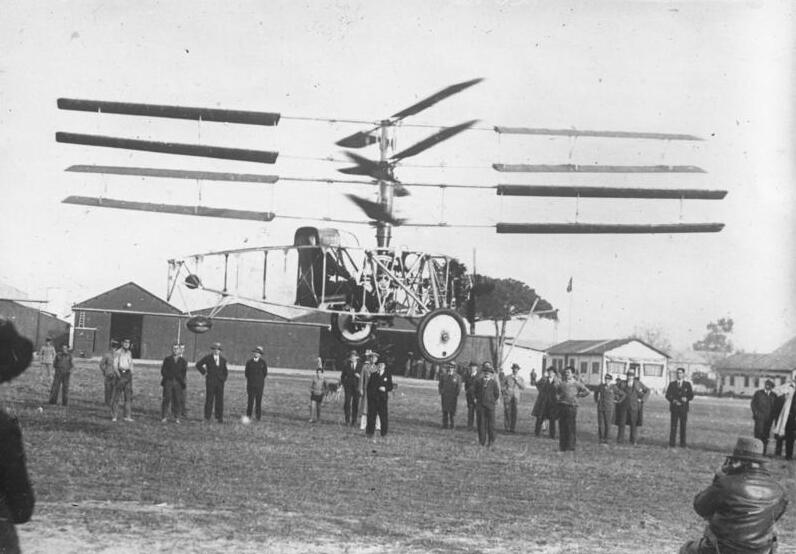
\includegraphics[width=0.55\textwidth]{Early_Coaxial.jpg}}
\end{wrapfigure}
To avoid this, multiple contra-rotating rotors which cancel out each others torque can be used. In early designs of the 1930s as many as 6 or 4 rotors were used, see Figure \ref{fig:Early}\cite{Pescara-1930} but this quickly proved impractical.
Therefore, the dual-rotor coaxial design established itself and is the only one still in use. The coaxial configuration provides several benefits over the single main rotor, but adds considerable engineering challenges. The aerodynamic interactions generated by the two rotors require additional considerations, and are still subject of ongoing research \cite{Richard-2010}. Some early experiments suggest a considerably higher power demand of a coaxial rotor configuration, when compared to an equivalent single rotor, \mbox{see Figure \ref{fig:Plot}} \cite{leishman-2000}. The advance ratio $\mu$ on the x-axis is the proportion of the airspeed $V_\infty$ to the rotor tip velocity $\Omega r$:
\begin{math}
    \mu = \frac{V_\infty}{\Omega r}
\end{math}. 
\begin{wrapfigure}[17]{R}[0pt]{0pt}
    \captionbox{\label{fig:Plot}\textit{Power requirement of a coaxial helicopter (black) against those of a single rotor one (red).}}
    {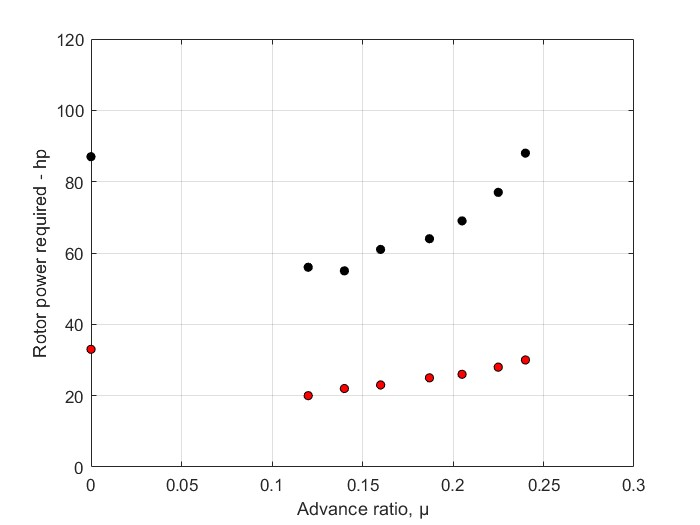
\includegraphics[width=0.4\textwidth]{Plot.jpg}}
\end{wrapfigure}

This finding has however been contested by others, who have found a coaxial rotor to need 5\% less power for a given thrust than a single rotor in hover and "less power" in forward flight \cite{Coleman-1997}.
One definite advantage of coaxial helicopters is the lift distribution over the rotor assembly in forward flight. Using a single rotor the retreating airfoil is experiencing lower relative air speed. This causes asymmetric lift distribution over the rotor area, which can be canceled out in a coaxial design, where one rotors retreating blade is necessarily the others advancing one. This was most notably used in the \hypertarget{Sikorsky}{Sikorsky S-69/X-59 Advancing Blade Concept} \cite{Coleman-1997}. Above certain velocities, the asymmetric speed distribution over the rotor requires an increasingly high angle of attack $\alpha$ on the retreating blade, which eventually causes dynamic stall, the same is true for too high airspeed causing a stall on the advancing blade. These "never exceed speeds" are higher on coaxial helicopters.
The mechanical complexity of the coaxial rotor and swashplate assembly is a major downside of the coaxial configuration, requiring both more maintenance than single rotors already do and more complicated design and manufacturing. 
\newpage
Yaw control is also more complicated, and usually solved through change of the angle of attack $\alpha$ of the individual rotors, producing a reaction torque and yaw control, see Figure \ref{fig:Yaw}. This mechanism also makes for additional engineering challenges.

\begin{wrapfigure}[15]{l}{220pt}
    \captionbox{\label{fig:Yaw}\textit{Yaw control in a coaxial rotor system. The imbalance of $D_1$ and $D_2$ creates torque.}}
    {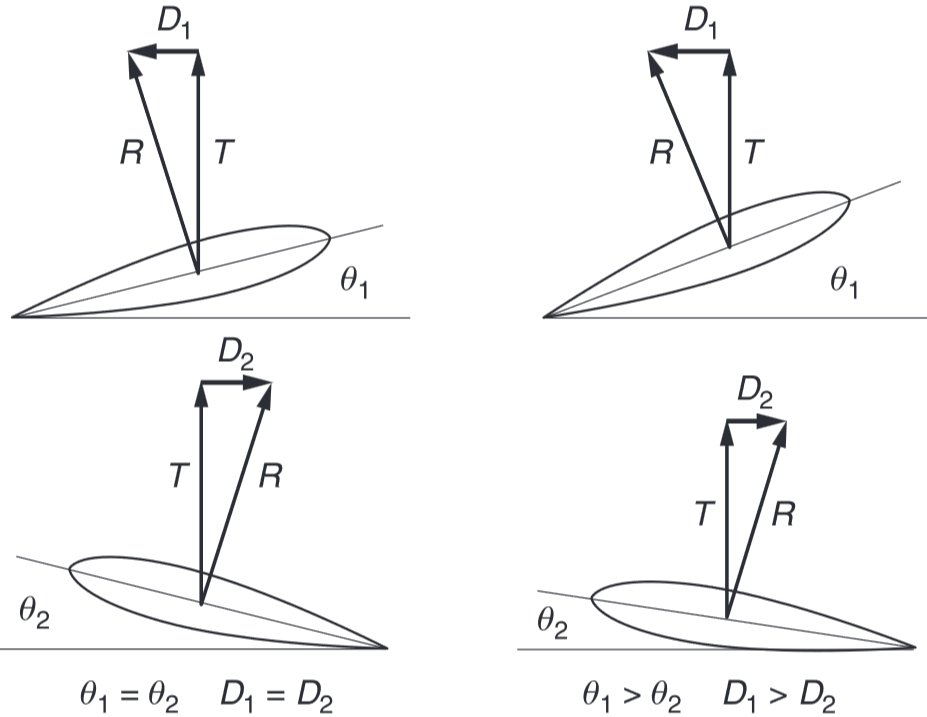
\includegraphics[width=0.4\textwidth]{Yawcontrol.png}}
\end{wrapfigure}
The obvious mechanical benefit of a coaxial helicopter is the complete lack of a tail rotor and associated parts. This allows a reduction in weight and size, the latter a main reason for the Soviet Navy to heavily utilize the coaxial helicopters made by the Kamov Design Bureau, since hangar volume on ships is often heavily limited. For reasons of yaw stability, coaxial helicopters do require \emph{some} form of tail appendage, but this can be solved with simple vertical stabilizers, at the cost of some additional drag. The total drag of coaxial helicopters is also increased by the taller swashplate assembly and rotor shaft structure, a major efficiency drawback. 

\section{Conclusion\label{Conc}}
Coaxial rotors have been built since the early beginnings of helicopter flight, and continue to be built and flown. With both NASA's \emph{Ingenuity} UAV\footnote{Unmanned Aerial Vehicle} on Mars and prototypes for the US Army's "Future Long-Range Assault Aircraft" competition utilizing a double rotor coaxial setup, it is clear that the advantages listed in section\ref{Main} will keep the design relevant, if niche, for future developments, especially as design challenges that previously hindered this design become more easily solvable using modern technology and materials. A potential future development is also a continuation of the principles in the Sikorsky Advancing Blade Concept, previously mentioned \hyperlink{Sikorsky}{here}, using coaxial rotors in a compound helicopter, to achieve a high efficiency combination of both airplane and helicopter, reaching higher speeds while maintaining vertical take-off capabilities. 

\printbibliography

\end{document}